\documentclass{article}

\usepackage[bib,bibstyle=ieee,bibargs={sorting=none},smalltitle,code,margin=0.95in]{shorthand}
\usepackage{pgfplots} \pgfplotsset{compat=1.16}
\usepackage{subfig}

\addbibresource{Report.bib}

\setcounter{secnumdepth}{0}

\title{Solving Partial Differential Equations using a Deep Neural Network}
\author{Hunter Damron}
\date{7 May 2019}

\def\model{may6}

\begin{document}
  \maketitle

  \section{Introduction}
    In recent years, the neural network has become a popular tool for a wide variety of applications from image classification~\cite{lenet5} to stock market prediction~\cite{stock}. Neural networks, in general, are used to approximate a partially known function using linear algebra often combined with a nonlinear component. The network contains weight and bias matrices which are gradually adjusted to better represent the function during a training process. Although the idea for the neural network has existed for many years as a model of neural activity, it gained popularity as a computational tool with Rosenblatt's perceptron~\cite{rosenblatt}. Cybenko shows that neural networks, although simple in nature, can be used to approximate any function~\cite{approx}.

  \section{Problem Statement}
    This paper presents a neural network used to approximate a partial differential equation $u(x,t)$ on the domain $x \in [0,1], t \in [0,T]$ with $T=2$. The network is then extrapolated to $T=10$. The value of $u$ is subject to the constraints
    \begin{subequations}\label{eqn:pde}
    \begin{gather}
      u(x,0) = \sin(4 \pi x) \label{eqn:x} \\
      u(0,t) = u(1,t) = 0 \label{eqn:t} \\
      \delbdt{u} = D \delbdx[2]{u} + \beta u \label{eqn:de}
    \end{gather}
    \end{subequations}
    where $D = \beta = 1$.

    The network approximation is compared against the analytical solution\footnote{Because I have no experience on solving differential equations and they are not in the scope of this course, the analytical solution is provided by Matthew Clapp.}
    \begin{equation} \label{eqn:sol}
      u(x,t) = \sin(4 \pi x) e^{ct} \text{ where } c = 1 - 16 \pi^2
    \end{equation}
    which is verified as a solution by
    \begin{subequations}
      \begin{gather}
        u(x,0) = \sin(4 \pi x) e^{c \cdot 0} = \sin(4 \pi x) \cdot 1 = \sin(4 \pi x) \text{\quad(satisfies \ref{eqn:x})} \\
        u(0,t) = \sin(4 \pi \cdot 0) e^{ct} = \sin(0) e^{ct} = 0 \cdot e^{ct} = 0 \text{\quad(satisfied \ref{eqn:t})}
      \end{gather}
      \begin{equation}
      \begin{split}
        \delbdx[2]{u} &= \deldx{4 \pi \cos(4 \pi x) e^{ct}} = -16 \pi^2 \sin(4 \pi x) e^{ct} = (c-1) u \\
        \delbdt{u} &= c \sin(4 \pi x) e^{ct} = c u = c u = (c-1) u + u = \delbdx[2]{u} + u \text{\quad(satisfies \ref{eqn:de})}.
      \end{split}
      \end{equation}
    \end{subequations}

  \bdef{x} \bdef{t} \bdef{X} \caldef{U}
  \section{Procedure}
      \hdef{u}
      \def\<{\left\langle}
      \def\>{\right\rangle}
      The neural network used in this paper takes a two-dimensional input $\< x,t \> \in \R^2$ and produces a one-dimensional output $\hu \in \R$ with three hidden layers each of width 80. The choice of the number and width of hidden layers was found experimentally to be reasonable. The $\tanh$ function was used as an activation because of its differentiable and symmetric nature.

      For estimating the cost of the model, the constraints of Equations~\ref{eqn:x}, \ref{eqn:t}, and~\ref{eqn:de} were reformulated into three residuals centered around 0
      \begin{subequations}
      \begin{gather}
        r_0(x) = u(x,0) - \sin(4 \pi x) \label{eqn:res_x} \\
        r_1(t_l, t_r) = u(0,t_l) + u(1,t_r) \label{eqn:res_t} \\
        r_2(x,t) = \delbdt{u} - D \delbdx[2]{u} - \beta u \label{eqn:res_de}
      \end{gather}
      \end{subequations}
      which are then minimized using the $MSE$ of each's $L_2$ norm for cost. Let $\bx^B \sim \calU(0,1)^k$, $\bt^L, \bt^R \sim \calU(0,T)^m$, and $\bX \sim (\calU(0,1) \times \calU(0,T) )^n$ be vectors of uniform random variables to be used as inputs. Given these inputs, the total cost is given by
      \begin{equation} \label{eqn:cost}
        J = \frac1k \sum_{i=0}^{k-1} r_0(\bx^B_i)^2
          + \frac1m \sum_{i=0}^{m-1} r_1(\bt^L_i, \bt^R_i)^2
          + \frac1n \sum_{i=0}^{n-1} r_2(\bX_i)^2.
      \end{equation}

      Training was conducted using the Adam optimization algorithm described in~\cite{adam} with a decaying learning rate. Adam was used because it requires only a learning rate and has provided decent results in a wide variety of applications. A simple gradient descent optimization was also able to give similar results but did not converge as quickly. The decaying learning rate was used to allow the network to quickly reach the correct order of magnitude before fine-tuning the structure. The weight matrices were initialized according to an element-wise random normal distribution and biases were initialized to 0. The input for each epoch was chosen randomly with 310 points -- 50 along the $t=0$ axis, 30 along the $x=0$ axis, 30 along the $x=1$ axis, and 200 in the center of the domain. The cost function was modified so the $r_0$ cost was multiplied by a weight of 10 because that constraint was found to be the most difficult to approximate.

      The TensorFlow framework~\cite{tf} provided the basis for all numerical calculations. Figure~\ref{fig:network} shows a schematic of the network described in this paper.

      \begin{figure}[!htbp]
        \centering
        \caption{Schematic of Neural Network (produced using NN-SVG~\cite{schematic})} \label{fig:network}
        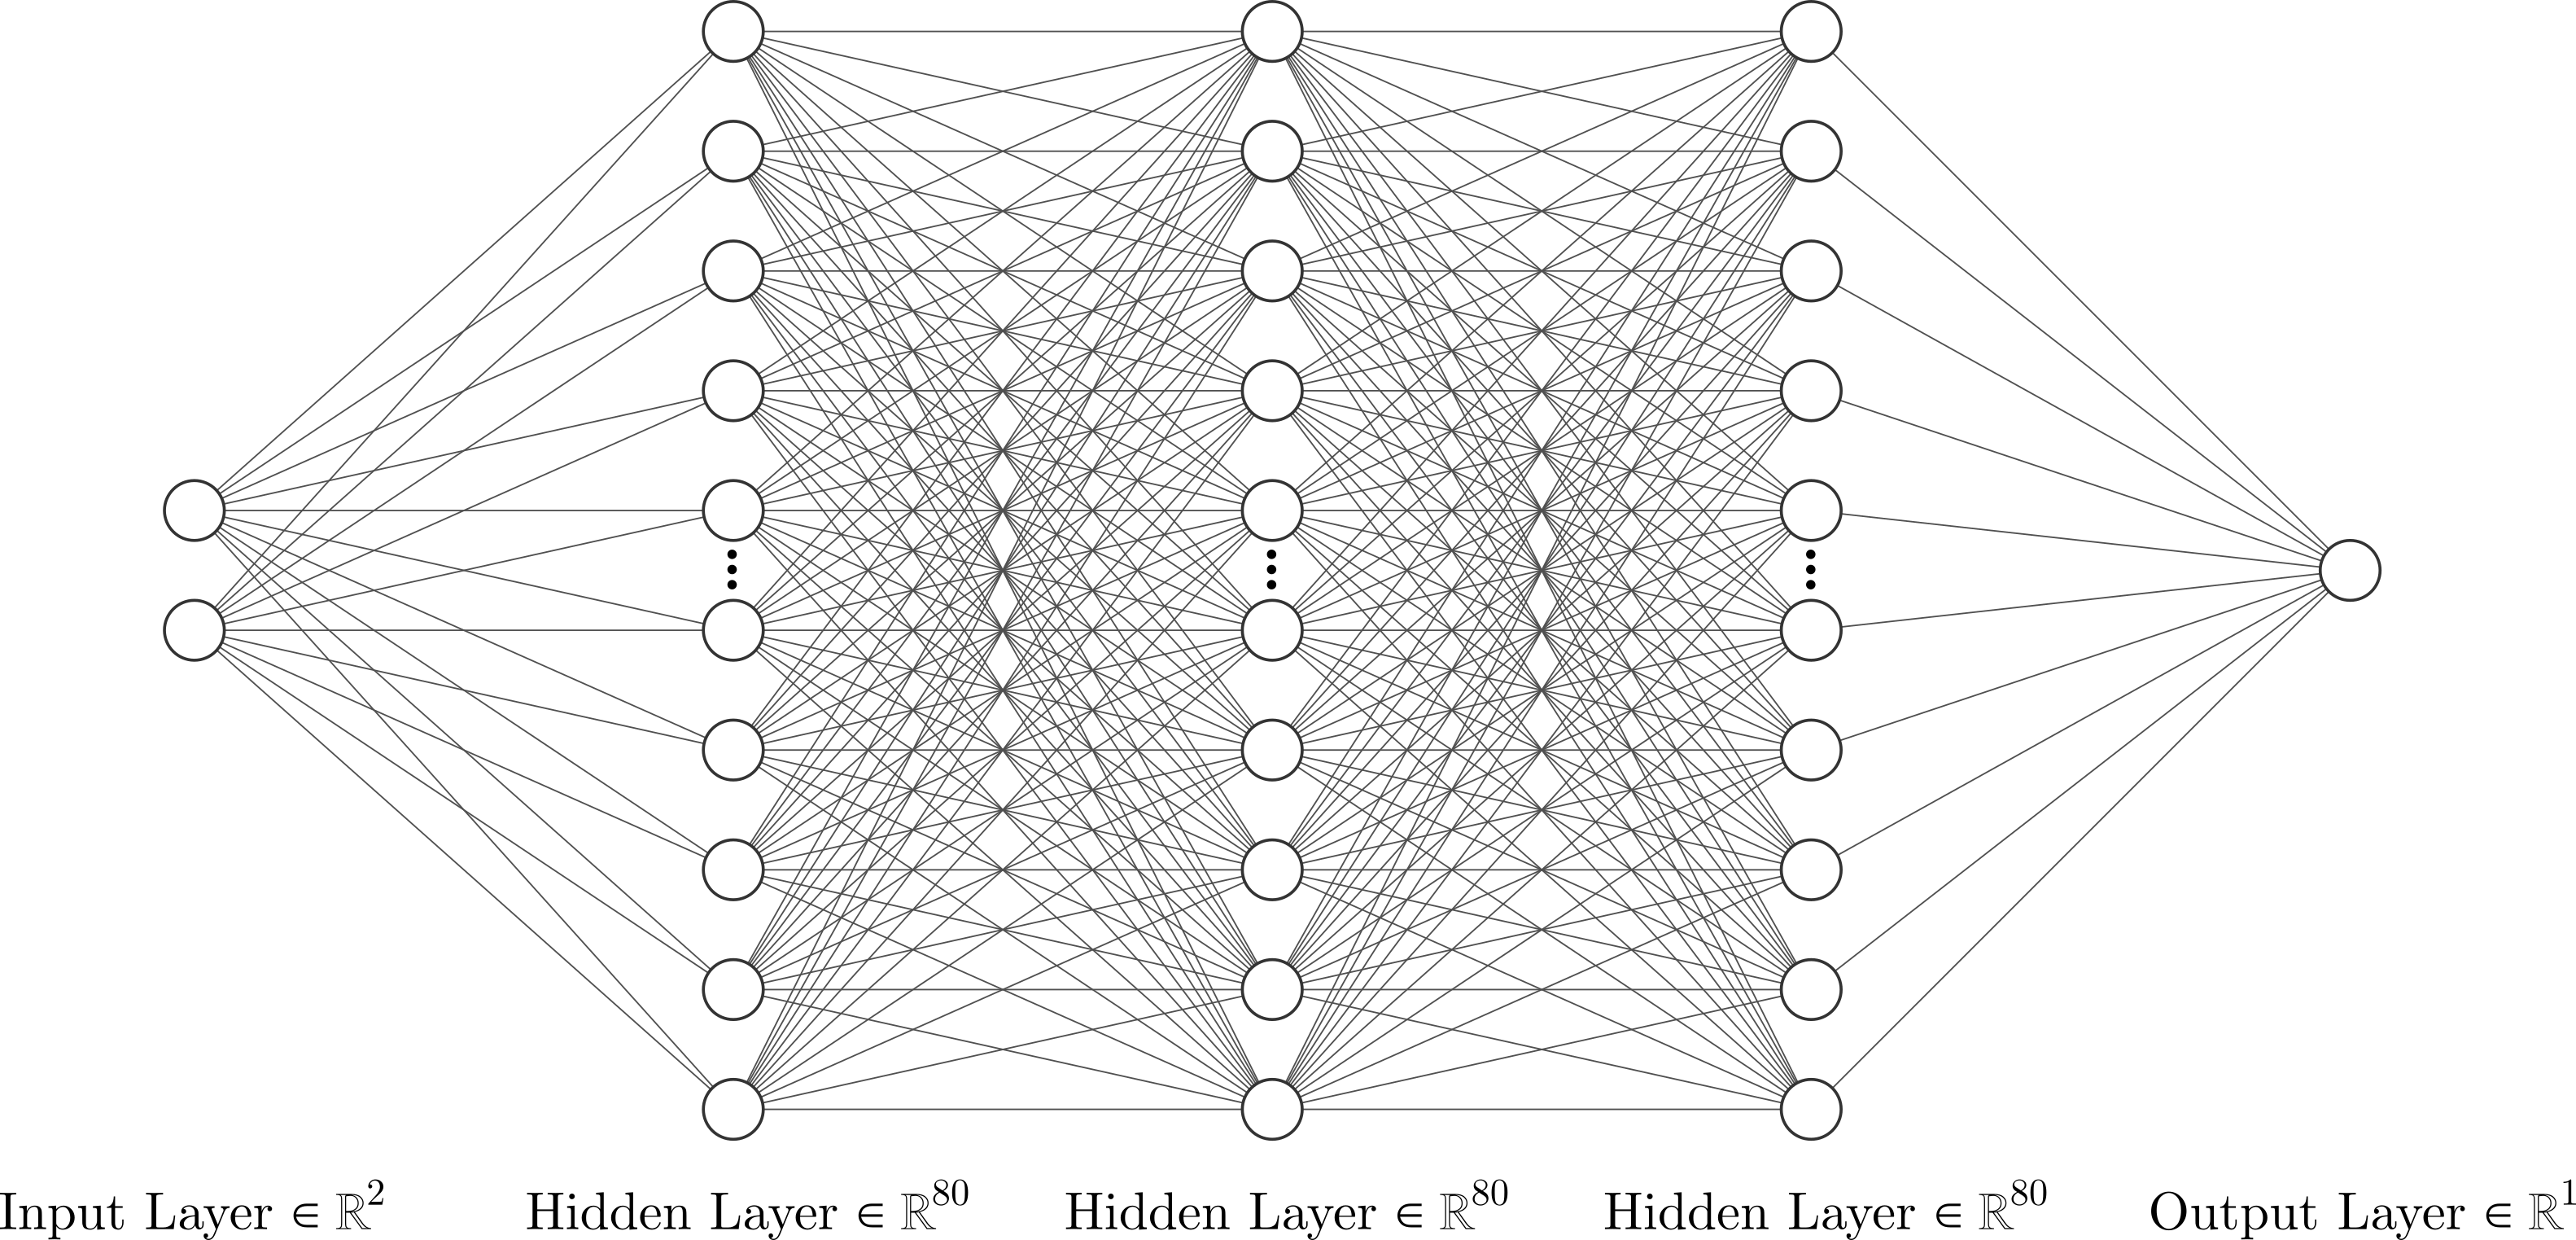
\includegraphics[width=0.9\linewidth]{figures/nn.png}
      \end{figure}
  \section{Results}
    The approximated function is shown beside the analytical solution in Figure~\ref{fig:plot} both in the training domain with $T=2$ and extrapolated to $T=10$. Figure~\ref{fig:loss} shows the error of the network through the epochs of training. The cost $J$ is the cost used for training defined in Equation~\ref{eqn:cost}. The error from the analytical solution is the $MSE$ of the network output compared to the solution given in Equation~\ref{eqn:sol}. This error is defined as
    \begin{equation}
      \hat{J} = \frac1n \sum_{i=0}^{n-1} (\hat{u}(\bX_i) - u(\bX_i))^2
    \end{equation}
    where $\hat{u}$ is the neural network. For this error, the input $\bX$ contains all input points not just those in the center of the domain. Note that only every third point is plotted in Figure~\ref{fig:loss}.

    \begin{figure}[!htbp]
      \centering
      \caption{Numerical and Analytical Solutions to $z = u(x,t)$} \label{fig:plot}
      \subfloat[$T=2$]{
        \includegraphics[width=0.8\textwidth]{figures/\model.png}
      }

      \subfloat[$T=10$]{
        \includegraphics[width=0.8\textwidth]{figures/\model-extrapolate.png}
      }
    \end{figure}

    \begin{figure}[!htbp]
      \centering
      \caption{Training Cost and Error during Training Process} \label{fig:loss}
      \begin{tikzpicture}
      \begin{axis}[
        xlabel={Epoch},
        ylabel={Error (logarithmically scaled)},
        ymode=log,
        width=0.7\textwidth
      ]
        \addplot[thick,mark=none,smooth] table[x expr={3*\coordindex}, y index=0,col sep=comma]{models/\model-losses-full-small.csv};
        \addplot[thick,mark=none,smooth,dotted] table[x expr={3*\coordindex}, y index=4,col sep=comma]{models/\model-losses-full-small.csv};
        \legend{Cost $J$, Error $\hat{J}$ from Analytical Solution};
      \end{axis}
      \end{tikzpicture}
    \end{figure}

  \section{Discussion}
    As seen in Figure~\ref{fig:plot}, the output of the neural network differs significantly from the analytical solution at the $t=0$ boundary but provides a good approximation everywhere else in the training domain. However, the network is able to learn the sinusoidal nature of the boundary and may be able to fully approximate the constraint given the right initial conditions. Unfortunately, as shown in Figure~\ref{fig:loss}, the learning appears to have reached a local minimum so further training would have had little effect. The comparison to the analytical solution also reflects a local minimum. It is possible that the network is not large enough to represent the full structure, but experimentation showed that deeper and wider networks only slowed learning with negligible improvement.

    When the neural network is extrapolated to $T=10$, its behavior is arbitrary and the network is no longer an approximate solution to the partial differential equation. This poor extrapolation is to be expected because the training process made no assertion about the network's behavior outside of the training domain. This inability to extrapolate demonstrates an important property of neural networks -- they are only able to make valid approximations within the domain of their training data.

  \printbibliography{}

  \appendix
  \section{Appendix}
  \setcounter{secnumdepth}{2}
  \renewcommand{\thesubsection}{\Alph{subsection}}
  \subsection{Network Implementation} \label{apx:code}
  \lstinputlisting{PartialDiffEq.py}
\end{document}
